\documentclass[11pt, oneside]{article}   	% use "amsart" instead of "article" for AMSLaTeX format
\usepackage{geometry}                		% See geometry.pdf to learn the layout options. There are lots.
\geometry{letterpaper}                   		% ... or a4paper or a5paper or ... 
%\geometry{landscape}                		% Activate for for rotated page geometry
%\usepackage[parfill]{parskip}    		% Activate to begin paragraphs with an empty line rather than an indent
\usepackage{graphicx}				% Use pdf, png, jpg, or eps§ with pdflatex; use eps in DVI mode
								% TeX will automatically convert eps --> pdf in pdflatex		
\usepackage{amssymb}
\usepackage[T1]{fontenc}
\usepackage{lmodern}
\usepackage{fixltx2e}
\usepackage{mathtools}

\title{Selected Exercises from Fundamentals of Database Systems}
\author{Andrew Kowalczyk}
\date{}

\begin{document}

\maketitle
I selected around 40 questions from the 6$^{th}$ edition of \textit{Fundamentals of Database Systems} by Ramez Elmasri and Shamkant Navathe. This was part of my requirement for my Introduction to Database Systems course taken in the Fall of 2013.

\section*{Chapter 1}
\addcontentsline{toc}{section}{Chapter 1}

\subsection*{1.8 Identify some informal queries and update operations that you would expect to apply to the database shown in Figure 1.2.}
\addcontentsline{toc}{subsection}{1.8}

\subsubsection*{Queries}

\begin{enumerate}
\item What are the prerequisites of the Database course?
\item Find the names of all students majoring in Mathematics.
\item Find the the transcript of the student named Brown.
\end{enumerate}

\subsubsection*{Updates}

\begin{enumerate}
\item Insert a new student in the database whose Name=Kowalczyk, Student\_number=25, Class=4, and Major=CS.
\item Change the grade that Brown received in Discrete Mathematics to a D.
\end{enumerate}

\subsection*{1.9 What is the difference between controlled and uncontrolled redundancy? Illustrate with examples.}
\addcontentsline{toc}{subsection}{1.9}
Redundancy is the term given when the same data is stored multiple times in several places in a database. If you look at Figure 1.5(a)  in the text, you can see that the name of the student with Student\_number=8 is Brown is stored multiple times. Redundancy is controlled when the database management system (DBMS) ensures that multiple copies of the same data are consistent. To illustrate this, let's say we are adding a new record with Student\_number=8 to be stored in the database of Figure 1.5(a). If we were to have uncontrolled redundancy, the DBMS would have no control over this. If we were to have controlled redundancy, the DBMS would ensure that Student\_name=Brown in that record.

\subsection*{1.10 Specify all the relationships among the records of the database shown in Figure 1.2.}
\addcontentsline{toc}{subsection}{1.10}
\begin{enumerate}
\item Every GRADE\_REPORT record is related to one STUDENT record and one SECTION record.
\item Every SECTION record is related to a COURSE record.
\item Every PREREQUISITE record relates two COURSE records. One being a course and the other being a prerequisite to that course.
\end{enumerate}

\subsection*{1.11 Give some additional views that may be needed by other user groups for the database shown in Figure 1.2.}
\addcontentsline{toc}{subsection}{1.11}
\begin{enumerate}
\item A view of each class section that groups all the students who took that section and their respective grade.
\item A view that gives the number of courses taken and the grade point average for each student.
\end{enumerate}

\subsection*{1.12 Cite some examples of integrity constraints that you think can apply to the database shown in Figure 1.2.}
\addcontentsline{toc}{subsection}{1.12}
\subsubsection*{Key constraints}
\begin{enumerate}
\item Student\_number must be unique for each STUDENT record.
\item Course\_number must be unique for each COURSE record.
\end{enumerate}

\subsubsection*{Referential integrity constraints}
\begin{enumerate}
\item The Course\_number in a SECTION record must also exist in some COURSE record.
\item The Student\_number in a GRADE\_REPORT record must also exist in some STUDENT record.
\end{enumerate}

\subsubsection*{Domain constraints}
\begin{enumerate}
\item Grades in a a given GRADE\_REPORT record must be one of these values: {A, B, C, D, F, I, W}.
\end{enumerate}
\pagebreak

\section*{Chapter 2}
\subsection*{2.12 Think of different users for the database shown in Figure 1.2. What types of applications would each user need? To which user category would each belong, and what type of interface would each need?}

\begin{enumerate}
  \item Students add and drop classes. Actions that they can do are as listed:
    \begin{enumerate}
       \item Register themselves in a section of a course
       \item Drop themselves from a section of a course 
    \end{enumerate}
  \item Registrar. They enter data of registration of students in sections of courses, and later enter the grades of the students. Actions that they can do are as listed:
    \begin{enumerate}
        \item Check whether a student who is registered in a course has the appropriate prerequisite courses
       \item Add a student to a section of a course
       \item Enter the student grades for a section
    \end{enumerate}
  \item Admissions. Their main application would be to enter newly accepted students into the database. Actions that they can do are as listed:
    \begin{enumerate}
    	\item Add students to the school's records
    \end{enumerate}
\end{enumerate}
\pagebreak

\section*{Chapter 3}
\subsection*{3.11 Suppose that each of the following Update operations is applied directly to the database state shown in Figure 3.6. Discuss all integrity constraints violated by each operation, if any, and the different ways of enforcing these constraints.}

In each of examples, the different ways of enforcing the constraints is listed in preferential order (\textit{i.e.} 1 is most preferred, 2 is less preferred, etc.).

\subsubsection*{(a) Insert <"Robert", "F", "Scott", "943775543", "1972-06-21", "2365 Newcastle Rd, Bellaire, TX", M, 58000, "888665555", 1> into EMPLOYEE.}
No constraints violated.

\subsubsection*{(b) Insert <"ProductA", 4, "Bellaire", 2> into PROJECT.}
 Since there is no tuple in the DEPARTMENT relation with DNUM=2, this insertion would violate referential integrity for that very reason. We can enforce the constraint with these options:
\begin{enumerate}
\item Rejecting the insertion
\item Changing the value of DNUM in the new PROJECT tuple to an existing DNUMBER value in the DEPARTMENT relation
\item Inserting a new DEPARTMENT tuple with DNUMBER=2
\end{enumerate}

\subsubsection*{(c) Insert <"Production", 4, "943775543", "2007-10-01"> into DEPARTMENT.}
Oh no! Since there already exists a DEPARTMENT tuple with DNUMBER=4, this would violate the key constraint. Enforcement of this constraint would happen by:
\begin{enumerate}
\item Rejecting the insertion
\item Changing the value of DNUMBER in the new DEPARTMENT tuple to a value that does not violate the key constraint
\end{enumerate}
Also, since there is no tuple in the EMPLOYEE relation with SSN="943775543", this insertion also happens to violate referential integrity. Let us enforce the constraint by either: 
\begin{enumerate}
\item Rejecting the insertion
\item Changing the value of MGRSSN to an existing SSN value in EMPLOYEE
\item Inserting a new EMPLOYEE tuple with SSN="943775543"
\end{enumerate}

\subsubsection*{(d) Insert <"677678989", NULL, "40.0"> into WORKS\_ON.}
Since PNO (part of the primary key of WORKS\_ON) is null, this violates entity integrity. We have these options to enforce this constraint:
\begin{enumerate}
\item Rejecting the insertion
\item Changing the value of PNO in the new WORKS\_ON tuple to a value of PNUMBER that exists in the PROJECT relation
\end{enumerate}
Since there is no tuple in the EMPLOYEE relation with SSN="677678989", this insertion would violate referential integrity. We may enforce the constraint by:
\begin{enumerate}
\item Rejecting the insertion
\item Changing the value of ESSN to an existing SSN value in EMPLOYEE
\item Inserting a new EMPLOYEE tuple with SSN="677678989"
\end{enumerate}

\subsubsection*{(e) Insert <"453453453","John","M","1990-12-12","spouse"> into DEPENDENT.}
Nope! Not a single constraint was violated.

\subsubsection*{(f) Delete the WORKS\_ON tuples with Essn = "333445555".}
No constraints violated in the making of this delete.

\subsubsection*{(g) Delete the EMPLOYEE tuple with Ssn = "987654321".}
Unfortunately, the employee trying to be deleted is referenced in the WORKS\_ON, DEPENDENT, DEPARTMENT, and EMPLOYEE relations. We can enforce such an abolishment by either:
\begin{enumerate}
\item Rejecting the deletion
\item Deleting all tuples in the WORKS\_ON, DEPENDENT, DEPARTMENT, and EMPLOYEE relations whose values for ESSN, ESSN, MGRSSN, and SUPERSSN, respectively, is equal to "987654321"
\end{enumerate}

\subsubsection*{(h) Delete the PROJECT tuple with Pname="ProductX".}
This deletion would completely violate referential integrity because two tuples exist in the WORKS\_ON relation that reference the tuple being deleted from PROJECT. Silly us,  let's enforce the constraint by:
\begin{enumerate} 
\item Rejecting the deletion
\item Deleting the tuples in the WORKS\_ON relation whose value for the primary key PNUMBER for the tuple being deleted from PROJECT with PNO=1
\end{enumerate}

\subsubsection*{(i) Modify the Mgr\_ssn and Mgr\_start\_date of the DEPARTMENT tuple with Dnumber = 5 to "123456789" and "2007-10-01", respectively.}
No violation of constraints.

\subsubsection*{(j) Modify the Super\_ssn attribute of the EMPLOYEE tuple with Ssn = "999887777" to "943775543".}
Goodness gracious, great balls of fire! Since there is no tuple in the EMPLOYEE relation with SSN="943775543", this update would violate referential integrity. In order to enforce this constraint, we can choose from:
\begin{enumerate}
\item Rejecting the deletion
\item Inserting a new EMPLOYEE tuple with SSN="943775543"
\end{enumerate}

\subsubsection*{(k) Modify the Hours attribute of the WORKS\_ON tuple with Essn = "999887777" and Pno = 10 to "5.0".}
No constraints violated.
\pagebreak

\section*{Chapter 4}
\addcontentsline{toc}{section}{Chapter 4}

\subsection*{4.9 How can the key and foreign key constraints be enforced by the DBMS? Is the enforcement technique you suggest difficult to implement? Can the constraint checks be executed efficiently when updates are applied to the database?}
\addcontentsline{toc}{subsection}{4.9}

In order to check efficiently for the key constraint, one can create an index on all of the attributes that form each primary or secondary key. Even before the new record is inserted, each index is searched to insure that no value currently exists in the index that matches the key value in the new record. If this is the case, the record is inserted successfully and we are happy.

In order to check efficiently for the foreign key constraint, the primary key is given an index for each referenced relation. Due to this, the check efficient enough for our purposes. Each time a new record is inserted in a referencing relation, we search the index for the primary key of the referenced relation. The value of its foreign key is used to accomplish this. The new record can be successfully inserted in the referencing relation if the referenced record exists. For the deletion of any given referenced record, an index on the foreign key of each of the referencing relations is very useful. We want to efficiently determine whether any records reference that given record. If the techniques described above do not exist, then, unfortunately, we must do linear searches to check for any of the above constraints. This would making the checks quite inefficient, and it would make us unhappy.


\subsection*{4.12 Specify the following queries in SQL on the database schema of Figure 1.2.}
\addcontentsline{toc}{subsection}{4.12}
\subsubsection*{(a) Retrieve the names of all senior students majoring in "CS" (computer sci- ence).}
\begin{lstlisting}[language=SQL]
SELECT Name 
FROM   STUDENT
WHERE  Major="CS"
    AND Class="4"
\end{lstlisting}

\subsubsection*{(b) Retrieve the names of all courses taught by Professor King in 2007 and 2008.}
\begin{lstlisting}[language=SQL]
SELECT Course_name
FROM   COURSE,
       SECTION
WHERE COURSE.Course_number=SECTION.Course_number
    AND Instructor="King"
    AND (Year="07" OR Year="08")
\end{lstlisting}

\subsubsection*{(c) For each section taught by Professor King, retrieve the course number, semester, year, and number of students who took the section.}
\begin{lstlisting}[language=SQL]
SELECT Course_number,
       Semester,
       Year,
       COUNT(*)
FROM   SECTION,
       GRADE_REPORT
WHERE Instructor="King"
    AND SECTION.Section_identifier=GRADE_REPORT.Section_identifier
GROUP BY Course_number, Semester, Year
\end{lstlisting}

\subsubsection*{(d) Retrieve the name and transcript of each senior student (Class = 4) majoring in CS. A transcript includes course name, course number, credit hours, semester, year, and grade for each course completed by the student.}
\begin{lstlisting}[language=SQL]
SELECT Name,
       C.Course_name,
       C.Course_number,
       Credit_hours,
       Semester,
       Year,
       Grade
FROM   STUDENT ST,
       COURSE C,
       SECTION S,
       GRADE_REPORT G
WHERE Class=4 
    AND Major="CS"
    AND ST.StudentNumber=G.StudentNumber
    AND G.Section_identifier=S.Section_identifier
    AND S.Course_number=C.Course_number
\end{lstlisting}
\pagebreak

\section*{Chapter 5}
\pagebreak

\section*{Chapter 6}

\subsection*{6.15. Show the result of each of the sample queries in Section 6.5 as it would apply to the database state in Figure 3.6.} 

\subsubsection*{Query 1: Find the name and address of all employees who work for the 'Research' department.}
\begin{center}
\begin{tabular}{ c | c | c }
  FNAME & LNAME & ADDRESS \\ \hline
  John & Smith & 731 Fondren, Houston, TX \\
  Franklin & Wong & 638 Voss, Houston, TX \\
  Ramesh &  Narayan & 975 Fire Oak, Humble, TX \\
  Joyce & English & 5631 Rice, Houston, TX \\
\end{tabular}
\end{center}

\subsubsection*{Query 2: For every project located in 'Stafford', list the project number, the controlling department number, and the department manager's last name, address, and birth date.}
\begin{center} 
\begin{tabular}{ c | c | c | c | c}
  PNUMBER & DNUM & LNAME & ADDRESS & BDATE \\ \hline
  10 & 4 & Wallace & 291 Berry, Bellaire, TX &20-JUN-31 \\
  30 & 4 & Wallace & 291 Berry, Bellaire, TX & 20-JUN-31 \\ 
\end{tabular}
\end{center}

\subsubsection*{Query 3: Find the names of all employees who work on all the projects controlled by department number 5.}
\begin{center}
\begin{tabular}{ c | c }
  LNAME & FNAME \\ \hline
\end{tabular}
\end{center}

\subsubsection*{Query 4: Make a list of project numbers for projects that involve an employee whose last name is 'Smith' as a worker or as a manager of the department that controls the project.}
\begin{center}
\begin{tabular}{ c }
  PNO \\ \hline
  1 \\
  2 \\
\end{tabular}
\end{center}

\subsubsection*{Query 5: List the names of all employees with two or more dependents.}
\begin{center}
\begin{tabular}{ c | c }
  LNAME & FNAME \\ \hline
  Smith & John \\
  Wong & Franklin \\
\end{tabular}
\end{center}

\subsubsection*{Query 6 List the names of employees who have no dependents.}
\begin{center}
\begin{tabular}{ c | c }
  LNAME & FNAME \\ \hline
  Zelaya & Alicia \\
  Narayan & Ramesh \\
  English & Joyce \\
  Jabbar & Ahmad \\
  Borg & James \\
\end{tabular}
\end{center}

\subsubsection*{Query 7: List the names of managers who have at least one dependent.}
\begin{center}
\begin{tabular}{ c | c }
  LNAME & FNAME \\ \hline
  Wallace & Jennifer \\
  Wong & Franklin \\
\end{tabular}
\end{center}

\subsection*{6.16 Specify the following queries on the COMPANY relational database schema shown in Figure 5.5, using the relational operators discussed in this chapter. Also show the result of each query as it would apply to the database state in Figure 3.6.}
I use the symbol $\sigma$ for SELECT, $\pi$ for PROJECT, $\rhd\lhd$ for EQUIJOIN, * for NATURAL JOIN, and $\mathfrak{F}$ for FUNCTION.

\subsubsection*{(a) Retrieve the names of employees in department 5 who work more than 10 hours per week on the "ProductX" project.}
\subsubsection*{Relational Operators}
EMP\_W\_X $\Leftarrow$ ( $\sigma$ \textsubscript{PNAME="ProductX"} (PROJECT)) $\rhd\lhd$ \textsubscript{(PNUMBER),(PNO)} (WORKS\_ON) \\
EMP\_WORK\_10 $\Leftarrow$ (EMPLOYEE) $\rhd\lhd$ \textsubscript{(SSN),(ESSN)} ( $\sigma$ \textsubscript{HOURS>10} (EMP\_W\_X)) \\
RESULT $\Leftarrow$ $\pi$ \textsubscript{LNAME,FNAME} ( $\sigma$ \textsubscript{DNO=5} (EMP\_WORK\_10))

\subsubsection*{Result}
\begin{center}
\begin{tabular}{ c | c }
  LNAME & FNAME \\ \hline
  Smith & John \\
  English & Joyce \\
\end{tabular}
\end{center}

\subsubsection*{(b) List the names of employees who have a dependent with the same first name as themselves.}
\subsubsection*{Relational Operators}
E $\Leftarrow$ (EMPLOYEE) $\rhd\lhd$ \textsubscript{(SSN,FNAME),(ESSN,DEPENDENT\_NAME)} (DEPENDENT)\\
R $\Leftarrow$ $\pi$ \textsubscript{LNAME,FNAME} (E)

\subsubsection*{Result}
\begin{center}
\begin{tabular}{ c | c }
  LNAME & FNAME \\ \hline
\end{tabular}
\end{center}

\subsubsection*{(c) Find the names of employees that are directly supervised by "Franklin Wong".}
\subsubsection*{Relational Operators}
WONG\_SSN $\Leftarrow$ $\pi$ \textsubscript{SSN} ( $\sigma$ \textsubscript{FNAME="Franklin" AND LNAME="Wong"} (EMPLOYEE))\\
WONG\_EMPS $\Leftarrow$ (EMPLOYEE) $\rhd\lhd$ \textsubscript{(SUPERSSN),(SSN)} (WONG\_SSN)\\
RESULT $\Leftarrow$ $\pi$ \textsubscript{LNAME,FNAME} (WONG\_EMPS)

\subsubsection*{Result}
\begin{center}
\begin{tabular}{ c | c }
  LNAME & FNAME \\ \hline
  Smith & John \\
  Narayan & Ramesh \\
  English & Joyce \\
\end{tabular}
\end{center}

\subsubsection*{(d) For each project, list the project name and the total hours per week (by all employees) spent on that project.}
\subsubsection*{Relational Operators}
PROJ\_HOURS(PNO,TOT\_HRS) $\Leftarrow$ \textsubscript{PNO} $\mathfrak{F}$ \textsubscript{SUM HOURS} (WORKS\_ON) \\
RESULT $\Leftarrow$ $\pi$ \textsubscript{PNAME,TOT\_HRS} ( (PROJ\_HOURS) $\rhd\lhd$ \textsubscript{(PNO),(PNUMBER)} (PROJECT) )

\subsubsection*{Result}  
\begin{center}
\begin{tabular}{ c | c }
  PNAME & TOT\_HRS  \\ \hline
  ProductX & 52.5 \\
  ProductY & 37.5 \\
  ProductZ & 50.0 \\
  Computerization & 55.0 \\
  Reorganization & 25.0 \\
  Newbenefits & 55.0 \\
\end{tabular}
\end{center}

\subsubsection*{(e) Retrieve the names of employees who work on every project.}
\subsubsection*{Relational Operators}
PROJ\_EMPS(PNO,SSN) $\Leftarrow$ $\pi$ \textsubscript{PNO,ESSN} (WORKS\_ON) \\
ALL\_PROJS(PNO) $\Leftarrow$ $\pi$ \textsubscript{PNUMBER} (PROJECT) \\
EMPS\_ALL\_PROJS $\Leftarrow$ PROJ\_EMPS $\div$ ALLPROJS \\
RESULT $\Leftarrow$ $\pi$ \textsubscript{LNAME,FNAME} (EMPLOYEE * EMP\_ALL\_PROJS)

\subsubsection*{Result}
\begin{center}
\begin{tabular}{ c | c }
  LNAME & FNAME \\ \hline
\end{tabular}
\end{center}

\subsubsection*{(f) Retrieve the names of employees who do not work on any project.}
\subsubsection*{Relational Operators}
ALL\_EMPS $\Leftarrow$ $\pi$ \textsubscript{SSN} (EMPLOYEE) \\
WORKING\_EMPS(SSN) $\Leftarrow$ $\pi$ \textsubscript{ESSN} (WORKS\_ON)\\
NON\_WORKING\_EMPS $\Leftarrow$ ALL\_EMPS - WORKING\_EMPS\\
RESULT $\Leftarrow$ $\pi$ \textsubscript{LNAME,FNAME} (EMPLOYEE * NON\_WORKING\_EMPS)

\subsubsection*{Result}
\begin{center}
\begin{tabular}{ c | c }
  LNAME & FNAME \\ \hline
\end{tabular}
\end{center}
\subsubsection*{(g) For each department, retrieve the department name and the average salary of all employees working in that department.}
\subsubsection*{Relational Operators}
DEPT\_AVG\_SALS(DNUMBER,AVG\_SAL) $\Leftarrow$ \textsubscript{DNO} $\mathfrak{F}$ \textsubscript{AVG SALARY} (EMPLOYEE)\\
RESULT $\Leftarrow$ $\pi$ \textsubscript{DNUMBER,AVG\_SAL} ( DEPT\_AVG\_SALS * DEPARTMENT )

\subsubsection*{Result}
\begin{center}
\begin{tabular}{ c | c }
  DNUMBER & AVG\_SAL  \\ \hline
  Research & 33250 \\
  Administration & 31000 \\
  Headquarters & 55000 \\
\end{tabular}
\end{center}

\subsubsection*{(h) Retrieve the average salary of all female employees.}
\subsubsection*{Relational Operators}
RESULT(AVG\_F\_SAL) $\Leftarrow$ $\mathfrak{F}$ \textsubscript{AVG SALARY} ( $\sigma$ \textsubscript{SEX="F"} (EMPLOYEE) )

\subsubsection*{Result}
\begin{center}
\begin{tabular}{ c }
  AVG\_F\_SAL \\ \hline
  31,000 \\
\end{tabular}
\end{center}

\subsubsection*{(i) Find the names and addresses of employees who work on at least one project located in Houston but whose department has no location in Houston.}
\subsubsection*{Relational Operators}
E\_P\_HOU(SSN) $\Leftarrow$ $\pi$ \textsubscript{ESSN} (WORKS\_ON $\rhd\lhd$ \textsubscript{(PNO),(PNUMBER)} ( $\sigma$ \textsubscript{PLOCATION="Houston"} (PROJECT)))\\
D\_NO\_HOU $\Leftarrow$ $\pi$ \textsubscript{DNUMBER} (DEPARTMENT) - $\pi$ \textsubscript{DNUMBER} ( $\sigma$ \textsubscript{DLOCATION="Houston"} (DEPARTMENT))\\
E\_D\_NO\_HOU $\Leftarrow$ $\pi$ \textsubscript{SSN} (EMPLOYEE  $\rhd\lhd$ \textsubscript{(PNO),(DNUMBER)} (D\_NO\_HOU))\\
RESULT\_EMPS $\Leftarrow$ E\_P\_HOU - E\_D\_NO\_HOU \\
RESULT $\Leftarrow$ $\pi$ \textsubscript{LNAME,FNAME,ADDRESS} (EMPLOYEE * RESULT\_EMPS)

\subsubsection*{Result}
\begin{center}
\begin{tabular}{ c | c | c}
  LNAME & FNAME  & ADDRESS \\ \hline
  Wallace & Jennifer & 291 Berry, Bellaire, TX \\
\end{tabular}
\end{center}

\subsubsection*{(j) List the last names of department managers who have no dependents.}
\subsubsection*{Relational Operators}
DEPT\_MANAGERS(SSN)<-- $\pi$ \textsubscript{MGRSSN} (DEPARTMENT) \\
EMPS\_WITH\_DEPENDENTS(SSN) $\Leftarrow$ $\pi$ \textsubscript{ESSN} (DEPENDENT) \\
RESULT\_EMPS $\Leftarrow$ DEPT\_MANAGERS - EMPS\_WITH\_DEPENDENTS \\
RESULT $\Leftarrow$ $\pi$ \textsubscript{LNAME,FNAME} (EMPLOYEE * RESULT\_EMPS)

\subsubsection*{Relational Operators}
\begin{center}
\begin{tabular}{ c | c }
  LNAME & FNAME \\ \hline
  Borg & James \\
\end{tabular}
\end{center}
\pagebreak

\section*{Chapter 7}
\pagebreak

\section*{Chapter 8}
\pagebreak

\section*{Chapter 9}
\addcontentsline{toc}{section}{Chapter 9}


\subsection*{9.3 Try to map the relational schema in Figure 6.14 into an ER schema. This is part of a process known as reverse engineering, where a conceptual schema is created for an existing implemented database. State any assumptions you make.}
\addcontentsline{toc}{subsection}{9.3}
\begin{center}
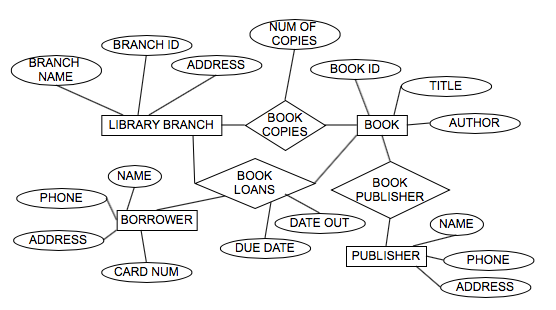
\includegraphics[width=15cm]{images/9-3.png}
\end{center}

Book authors, in this particular diagram, are represented as a multi-valued attribute of books.
\pagebreak

\section*{Chapter 10}

\end{document}  